\documentclass[aoas]{imsart}

\RequirePackage{amsthm,amsmath,amsfonts,amssymb,centernot,float,import,makeidx,subfiles, mathtools, epstopdf, hyperref, lscape, subcaption, accents, tabularx, threeparttable, varioref, longtable, natbib, graphicx, xr}

\usepackage[nokeyprefix]{refstyle}
% reference external document

\startlocaldefs
\theoremstyle{plain}
\newtheorem{axiom}{Axiom}
\newtheorem{claim}[axiom]{Claim}
\newtheorem{theorem}{Theorem}[section]
\newtheorem{lemma}[theorem]{Lemma}
\newtheorem{proposition}{Proposition}
\newcommand{\matr}[1]{\mathbf{#1}} % undergraduate algebra version
\newcommand{\mathbbm}[1]{\text{\usefont{U}{bbm}{m}{n}#1}} 
\theoremstyle{remark}
\newtheorem{remark}{remark}
\endlocaldefs
\usepackage{xr}
\usepackage{xcite}
\makeatletter
\newcommand*{\addFileDependency}[1]{% argument=file name and extension
  \typeout{(#1)}% latexmk will find this if $recorder=0 (however, in that case, it will ignore #1 if it is a .aux or .pdf file etc and it exists! if it doesn't exist, it will appear in the list of dependents regardless)
  \@addtofilelist{#1}% if you want it to appear in \listfiles, not really necessary and latexmk doesn't use this
  \IfFileExists{#1}{}{\typeout{No file #1.}}% latexmk will find this message if #1 doesn't exist (yet)
}
\makeatother

\newcommand*{\myexternaldocument}[1]{%
    \externaldocument{#1}%
    \addFileDependency{#1.tex}%
    \addFileDependency{#1.aux}%
}

\myexternaldocument{appendix-revised}

\begin{document}

\begin{frontmatter}

\title{Balancing weights for estimated region-level data: the effect of Medicaid Expansion on the uninsurance rate among states that did not expand Medicaid}
%\title{A sample article title with some additional note\thanksref{T1}}
\runtitle{Medicaid Expansion}
%\thankstext{T1}{A sample of additional note to the title.}

%%%%%%%%%%%%%%%%%%%%%%%%%%%%%%%%%%%%%%%%%%%%%%
%%Only one address is permitted per author. %%
%%Only division, organization and e-mail is %%
%%included in the address.                  %%
%%Additional information can be included in %%
%%the Acknowledgments section if necessary. %%
%%%%%%%%%%%%%%%%%%%%%%%%%%%%%%%%%%%%%%%%%%%%%%

\begin{aug}
\author[A]{\fnms{Max} \snm{Rubinstein}\ead[label = e1]{mrubinst@andrew.cmu.edu}},
\author[A]{\fnms{Amelia} \snm{Haviland}\ead[label = e2,mark]{amelia@andrew.cmu.edu}}, \and
\author[A]{\fnms{David} \snm{Choi}\ead[label = e3,mark]{davidch@andrew.cmu.edu}}
\address[A]{Carnegie Mellon University, Heinz College and Department of Statistics \& Data Science, \printead{e1,e2,e3}}
\end{aug}

\begin{flushleft}
We predict the average effect of Medicaid expansion on the non-elderly adult uninsurance rate among states that did not expand Medicaid in 2014 as if they had expanded their Medicaid eligibility requirements. Using American Community Survey data aggregated to the region level, we estimate this effect by finding weights that approximately reweights the expansion regions to match the covariate distribution of the non-expansion regions. Existing methods to estimate balancing weights often assume that the covariates are measured without error and do not account for dependencies in the outcome model. Our covariates have random noise that is uncorrelated with the outcome errors and our outcome model has state-level random effects inducing dependence between regions. To correct for the bias induced by the measurement error, we propose generating our weights on a linear approximation to the true covariates. This requires auxiliary data to estimate the variability of the measurement error. We also propose an objective function to reduce the variance of our estimator when the model errors follow our assumed correlation structure. Using this method, we estimate that Medicaid expansion would have caused a -2.33 (-3.54, -1.11) percentage point change in the adult uninsurance rate among states that did not expand Medicaid.
\end{flushleft}


\begin{keyword}
\kwd{Balancing weights}
\kwd{Medicaid expansion}
\kwd{measurement error}
\kwd{hierarchical data}
\end{keyword}

\end{frontmatter}
%%%%%%%%%%%%%%%%%%%%%%%%%%%%%%%%%%%%%%%%%%%%%%
%% Please use \tableofcontents for articles %%
%% with 50 pages and more                   %%
%%%%%%%%%%%%%%%%%%%%%%%%%%%%%%%%%%%%%%%%%%%%%%
%\tableofcontents

%%%%%%%%%%%%%%%%%%%%%%%%%%%%%%%%%%%%%%%%%%%%%%
%%%% Main text entry area:

\section{Introduction}

We study the effect of 2014 Medicaid expansion on the non-elderly adult uninsurance rates among states that did not expand Medicaid in 2014 as if they had expanded their Medicaid eligibility requirements. We use public-use survey microdata from annual American Community Survey (ACS) aggregated to the consistent public use microdata area (CPUMA) level, a geographic region that falls within states. We calculate weights that reweight expansion-state CPUMAs to approximately match the covariate distribution of CPUMAs in states that did not expand Medicaid in 2014. We then estimate our causal effect as the difference in means between the reweighted treated CPUMAs and the observed mean of the non-expansion CPUMAs. A key challenge is that our data consists of estimated covariates. The sampling variability in these estimates is a form of measurement error that may bias effect estimates calculated on the observed data. Additionally, CPUMAs fall within states and share a common policy-making environment. The data-generating process for the outcomes therefore may contain state-level random effects that can worsen the efficiency of standard estimation procedures. Our study contributes to the literature on balancing weights by proposing an approach to address both of these problems. We also contribute to the literature on Medicaid expansion by estimating the foregone coverage gains of Medicaid among states that did not expand Medicaid in 2014, which to our knowledge has not yet been directly estimated.

Approximate balancing weights are an estimation method in causal inference that grew out of the propensity score weighting literature. Rather than iteratively modeling the propensity score until the inverse probability weights achieve a desired level of balance, recent papers propose using optimization methods to generate weights that enforce covariate balance between the treated and control units (see, e.g., \cite{hainmueller2012entropy}, \cite{imai2014covariate}, \cite{zubizarreta2015stable}). From an applied perspective, there are at least four benefits of this approach: first, it does not require iterating propensity score models to generate satisfactory weights. Second, these methods (and propensity score methods generally) do not use outcomes in the modeling stage, mitigating the risk of cherry-picking model specifications. Third, these methods can constrain the weights to prevent extrapolation from the data, reducing model dependence \cite{zubizarreta2015stable}. Finally, the estimates are more interpretable: by making the comparison group explicit, it is easy to communicate exactly which units contributed to the counterfactual estimate.

Most proposed methods in this literature assume that the covariates are measured without error. For our application we assume that our covariates are measured with mean-zero additive error. This error could potentially bias standard estimation procedures. As a first contribution, we therefore propose generating our weights as a function of a linear approximation to the true covariate values, using an idea from the measurement error literature known as ``regression-calibration'' (see, e.g., \cite{carroll2006measurement}, \cite{gleser1992importance}). This method requires access to an estimate of the measurement error covariance matrix, which we estimate using the ACS microdata. The theoretic consistency of these estimates also requires several assumptions, including that the covariate measurement errors are uncorrelated with any errors in the outcome model, the outcome model is linear, and the data are gaussian. The first assumption is reasonable for our application since the covariates are measured on a different cross-sectional survey than our outcomes. The second is strong but somewhat relaxed because we prevent our weights from extrapolating beyond the support of the data. The third can be relaxed to obtain consistent estimates using ordinary least squares (OLS), but unfortunately not with our proposed method. Despite appearing costly, we show in Section~\ref{ssec:methodsmsrment} that this tradeoff is likely worth it in our application.

As a second contribution, we propose modifying the Stable Balancing Weights (SBW) objective (\cite{zubizarreta2015stable}) to account for possible state-level dependencies in our outcome model. We assume that the errors are homoskedastic with constant positive equicorrelation, though our general approach could easily accommodate other assumed correlation structures. In a setting without measurement error, we show that this modification can improve the efficiency of the resulting estimates. We also connect these weights to the implied regression weights from Generalized Least Squares (GLS). Our overall approach provides a general framework that can be used by other applied researchers who wish to use balancing weights to estimate causal effects when their data are measured with error and/or the model errors are dependent.\footnote{Our approach also relates to the ``synthetic controls'' literature (see, e.g., \cite{abadie2010synthetic}). Synthetic controls are a popular balancing weights approach frequently used in the applied economics literature to estimate treatment effects on the treated (ETT) for region-level policy changes when using time series cross sectional data. Our application uses a similar data structure; however, we instead consider the problem of estimating the ETC. In contrast to much of the synthetic controls literature, which assumes that the counterfactual outcomes follow a linear factor model, we also assume no unmeasured confounding and a linear outcome model.}

Section 2 begins with a more detailed overview of the policy problem, and then defines the study period, covariates, outcome, and treatment. Section 3 discusses our methods, including outlining our identification, estimation, and inferential procedures. Section 4 presents our results. Section 5 contains a discussion of our findings, and Section 6 contains a brief summary. The Appendices contain proofs, summary statistics, and additional results.

\section{Policy Problem and Data}

\subsection{Policy Problem Statement}

Under the Affordable Care Act (ACA), states were required to expand their Medicaid eligibility requirements by 2014 to offer coverage to all adults with incomes at or below 138 percent of the federal poverty level (FPL). The United States Supreme Court ruled this requirement unconstitutional in 2012, allowing states to decide whether to expand Medicaid coverage. In 2014, twenty-six states and the District of Columbia expanded their Medicaid programs. From 2015 through 2020, an additional twelve states elected to expand their Medicaid programs. In July 2021, Oklahoma and Missouri voted to expand their programs.\footnote{https://www.kansascity.com/news/politics-government/article250170945.html} Legislatures in other traditionally conservative states, including Alabama, North Carolina, and Wyoming also reportedly were considering expanding their programs in Spring 2021.\footnote{https://www.nbcnews.com/politics/politics-news/changed-hearts-minds-biden-s-funding-offer-shifts-medicaid-expansion-n1262229} The effects of Medicaid expansion on various outcomes, including uninsurance rates, mortality rates, and emergency department use, have been widely studied, primarily by using the initial expansions in 2014 and 2015 to define expansion states as ``treated'' states and non-expansion states as ``control'' states (see, e.g., \cite{courtemanche2017early}, \cite{wherry2016early}, \cite{ladhania2021effect}).

Medicaid enrollment is not automatic, and take-up rates have historically varied across states. This variation is partly a function of state discretion in administering programs: for example, program outreach, citizenship verification policies, and application processes differ across states (\cite{courtemanche2017early}). Estimating how Medicaid eligibility expansion actually affects the number of uninsured individuals is therefore not obvious. This is also important because many effects are mediated largely through reducing the number of uninsured individuals. Existing studies have estimated that Medicaid expansion reduced the uninsurance rate between three and six percentage points on average among states that expanded Medicaid. These estimates differed depending on the data used, specific target population, study design, and level of analysis (see, e.g., \cite{kaestner2017effects}, \cite{courtemanche2017early}, \cite{frean2017premium}). However, none of these studies have directly estimated the average treatment effect on the controls (ETC). 

We believe that the ETC may differ from the ETT. Every state had different coverage policies prior to 2014, and non-expansion states tended to have less generous policies than expansion states. ``Medicaid expansion'' therefore represents a set of treatments of varying intensities that are distributed unevenly across expansion and non-expansion states. Averaged over the non-expansion states, which tended to have less generous policies and higher uninsurance rates prior to Medicaid expansion, we might expect the average effect to be larger in absolute magnitude than among the expansion states, where ``Medicaid expansion'' on average reflected smaller policy changes.\footnote{As a part of our analysis strategy, we limit our pool of expansion states to those where the policy changes were comparable to the non-expansion states. We also control for pre-treatment uninsurance rates (see Section~\ref{sssec:txassign}).} Even limited to states with equivalent coverage policies prior to 2014 we still might expect the ETT to differ from the ETC. For example, all states that were entirely controlled by the Democratic Party at the executive and legislative levels expanded their Medicaid programs, while only states where the Republican Party controlled at least part of the state government failed to expand their programs. Prior to the 2014 Medicaid expansion, \cite{sommers2012understanding} found that conservative governance was associated with lower Medicaid take-up rates. This might reflect differences in program implementation, which could serve as effect modifiers for comparable policy changes.\footnote{Interestingly, \cite{sommers2012understanding} also find that the association between conservative governance and lower take-up rates prior to 2014 existed even after controlling for a variety of factors pertaining to state-level policy administration decisions. They posit that this may reflect cultural conservatism: people in conservative states are more likely to view enrollment in social welfare programs negatively, and therefore be less likely to enroll.} These factors may then attenuate the effects of Medicaid expansion averaged over non-expansion states relative to expansion states.

The ETC is also interesting in its own right: to the extent the goal of studying Medicaid expansion is to understand the foregone benefits (or potential harms) of Medicaid among non-expansion states, the ETC is the relevant quantity of interest. Authors have previously made claims about the ETC without directly estimating it. For example, \cite{miller2019medicaid} use their estimates of the ETT to predict that had non-expansion states expanded Medicaid, they would have seen 15,000 fewer deaths during their study period. From a policy analysis perspective, we emphasize that researchers should estimate the ETC directly when it answers a substantive question of interest. We therefore contribute to the literature on Medicaid expansion by directly estimating this quantity.

\subsection{Data Source and Study Period}\label{ssec:data}

Our primary data source is the annual household and person public use microdata files from the ACS from 2011 through 2014. The ACS is an annual cross-sectional survey of approximately three million individuals across the United States. The public use microdata files include information on individuals in geographic areas greater than 65,000 people. The smallest geographic unit contained in these data are public-use microdata areas (PUMAs), arbitrary boundaries that nest within states but not within counties or other more commonly used geographic units. One limitation of these data is a 2012 change in the PUMA boundaries, which do not overlap well with the previous boundaries. As a result, the smallest possible geographic areas that nest both PUMA coding systems are known as consistent PUMAs (CPUMAs). The United States contains 1,075 total CPUMAs, with states ranging from having one CPUMA (South Dakota, Montana, and Idaho) to 123 CPUMAs (New York). Our primary dataset (discussed further in Section~\ref{sssec:txassign}) contains 929 CPUMAs among 46 states. The average total number of sampled individuals per CPUMA across the four years is 1,001; the minimum number of people sampled was 334 and the maximum is 23,990. We then use the survey weights to aggregate the microdata to the CPUMA level.  

This aggregation naturally raises concerns about measurement error and hierarchy. Any CPUMA-level variable is an estimate, leading to concerns about measurement error. The hierarchical nature of the dataset -- CPUMAs within states -- leads to concerns about geographic dependence.

We begin our study period in 2011 following \cite{courtemanche2017early}, who note that several other aspects of the ACA were implemented in 2010 -- including the provision allowing for dependent coverage until age 26 and the elimination of co-payments for preventative care -- and likely induced differential shocks across states. We also restrict our post-treatment period to 2014. As a result, we avoid additional assumptions required for identification given that several states expanded Medicaid in 2015, including Indiana, Michigan, and Pennsylvania.

\subsection{Treatment assignment} \label{sssec:txassign}

Reducing the concept of ``Medicaid expansion'' to a binary treatment simplifies a more complex reality. There are at least three reasons to be cautious about this simplification. First, states differed substantially in their Medicaid coverage policies prior to 2014. Given perfect data we might ideally consider Medicaid expansion as a continuous treatment with values proportional to the number of newly eligible individuals. The challenge is correctly identifying newly eligible individuals in the data (see \cite{frean2017premium}, who attempt to address this). Second, \cite{frean2017premium} note that five states (California, Connecticut, Minnesota, New Jersey, and Washington) and the District of Columbia adopted partial limited Medicaid expansions prior to 2014. The ``2014 expansion'' therefore actually occurred in part prior to 2014 for several states.\footnote{\cite{kaestner2017effects} and \cite{courtemanche2017early} also consider Arizona, Colorado, Hawaii, Illinois, Iowa, Maryland, and Oregon to have had early expansions.} Finally, timing is an issue: among the states that expanded Medicaid in 2014, Michigan's expansion did not go into effect until April 2014, while New Hampshire's expansion did not occur until September 2014.

Our primary analysis excludes New York, Vermont, Massachusetts, Delaware, and the District of Columbia from our pool of expansion states because these states had comparable Medicaid coverage policies prior to 2014 and therefore reflect invalid comparisons (\cite{kaestner2017effects}). We also exclude New Hampshire because it did not expand Medicaid until September 2014. While Michigan expanded Medicaid in April 2014, we leave this state in our pool of ``treated'' states. We consider the remaining expansion states, including those with early expansions, as ``treated'' and the non-expansion states, including those that later expanded Medicaid, as ``control'' states. We later consider the sensitivity of our results to these classifications by removing the early expansion states indicated by \cite{frean2017premium}. Our final dataset contains data for 925 CPUMAs, with 414 CPUMAs among 24 non-expansion states and 511 CPUMAs among 21 expansion states. When we exclude the early expansion states, we are left with 292 CPUMAs across 16 expansion states. We provide a complete list of states by Medicaid expansion classification in Appendix~\ref{app:sumstats}.

\subsection{Outcome}

Our outcome is the non-elderly adult uninsurance rate in 2014. While take-up among the Medicaid-eligible population is a more natural outcome, we choose the non-elderly adult uninsurance rate for two reasons, one theoretic and one practical. First, Medicaid eligibility post-expansion is likely endogenous: Medicaid expansion may affect an individual's income and poverty levels, which in general define Medicaid eligibility. Second, we can better compare our results with the existing literature, including \cite{courtemanche2017early}, who also use this outcome. One drawback is that the simultaneous adoption of other ACA provisions by all states in 2014 also affects this outcome. As a result, we only attempt to estimate the effect of Medicaid expansion in 2014 in the context of this changing policy environment. We discuss this further in Sections~\ref{ssec:estimand} and ~\ref{ssec:identification}. 

\subsection{Covariates}

We choose our covariates to approximately align with those considered in \cite{courtemanche2017early} and that are likely to be potential confounders. Specifically, using the ACS public use microdata, we calculate the unemployment and uninsurance rates for each CPUMA from 2011 through 2013. We also estimate a variety of demographic characteristics averaged over this same time period, including percent female, white, married, Hispanic ethnicity, foreign-born, disabled, students, and citizens. We estimate the percent in discrete age categories, education attainment categories, income-to-poverty ratio categories, and categories of number of children. Finally, we calculate the average population growth and number of households to adults. We provide a more extensive description of our calculation of these variables in Appendix~\ref{app:adjustmentdetails}.

In addition to the ACS microdata we use 2010 Census data to estimate the percentage living in an urban area for each CPUMA. Lastly, we include three state-level covariates reflecting the partisan composition of each state's government in 2013 using data obtained from the National Conference of State Legislatures (NCSL). These include an indicator for states with a Republican governor, Republican control over the lower legislative chamber, and Republican control over both legislative chambers and the governorship.\footnote{Nebraska is the only state with a unicameral legislature and the legislature is technically non-partisan. We nevertheless classified them as having Republican control of the legislature for this analysis.} 

\section{Methods}\label{sec:methods}

In this section we present our causal estimand, identifying assumptions, estimation strategy, and inferential procedure. Our primary methodological contributions are contained in the subsection on estimation. We begin by outlining notation.

\subsection{Notation}
We let $s$ index states, and $c$ index CPUMAs within states. Let $m$ denote the number of states, $p_s$  the number of CPUMAs in state $s$, and $n = \sum_{s=1}^m p_s$ the total number of CPUMAs. For each state $s$, let $A_s$ denote its treatment assignment according to the discussion given in Section \ref{sssec:txassign}, with $A_s = 1$ indicating treatment and $A_s=0$ indicating control. For each CPUMA $c$ in state $s$, let $Y_{sc}$ denote the outcome of interest, its uninsurance rate in 2014; let $X_{sc}$ denote a q-dimensional covariate vector; and let $A_{sc} = A_{s}$ denote its treatment status. We assume potential outcomes (\cite{rubin2005causal}), defining a CPUMA's potential uninsurance under treatment by $Y^1_{sc}$, and under control by $Y^0_{sc}$. Finally, we let $n_1$ and $n_0$ denote the number of treated and control CPUMAs, and define $m_1$ and $m_0$ analagously for states.

Given a set $x$ indexed over CPUMAs, let $x_{A=1}$ and $x_{A=0}$ denote its subsets corresponding to the treated and control units
\[ x_{A=a} = \{x_{sc}: A_{sc}=a\}\]
so that, for example, $X_{A=0}$ corresponds to the covariates of the control units, and $Y_{A=1}^a$ corresponds to the potential outcomes $Y^a$ of the treated units, and so forth. Let $\bar{x}_a$ (which abbreviates $\bar{x}_{A=a}$) denote the average over units with treatment assignment $A_{sc} = a$:

\begin{align*}
	\bar{x}_a & = \frac{1}{n_a} \sum_{sc: A_{sc}=a} x_{sc}
\end{align*}
so that, for example, $\bar{Y}_0^1$ represents the average potential outcome under treatment for the control units.

\subsection{Estimand} \label{ssec:estimand}

We define the causal estimand $\psi$

\begin{align} \label{eqn:psi}
    \psi &= n_0^{-1} \sum_{sc: A_{sc}=0} \mathbb{E}\left[ Y_{sc}^1 - Y_{sc}^0 | X_{sc}\right] = \mathbb{E}[\bar{Y}_0^1 - \bar{Y}_0^0 \mid X_{A=0}] \\ 
    &= \psi_0^1 - \psi_0^0
\end{align}
where $\psi_0^a$ denotes the expectation $\mathbb{E}[\bar{Y}_0^a \mid X_{A=0}]$. The estimand $\psi$ represents the expected treatment effect on non-expansion states conditioning on the observed covariate distribution of the non-expansion states (see, e.g., \cite{imbens2004nonparametric}). The challenge is that we do not observe the counterfactual outcomes for non-expansion CPUMAs had their states expanded their Medicaid programs. We therefore require causal assumptions to identify this counterfactual quantity using our observed data.\footnote{As noted previously, the 2014 Medicaid expansion occurred simultaneously with the implementation of several other major ACA provisions, including (but not limited to) the creation of the ACA-marketplace exchanges, the individual mandate, health insurance subsidies, and community-rating and guaranteed issue of insurance plans (\cite{courtemanche2017early}). Almost all states broadly implemented these reforms beginning January 2014. Conceptually we think of the other ACA components as a state-level treatment ($R$) separate from Medicaid expansion ($A$). Our total estimated effect may also include interactions between these policy changes; however, we do not attempt to separately identify these effects. Without further assumptions, we therefore cannot generalize these results beyond 2014.} 

\subsection{Identification} \label{ssec:identification}

We appeal to the following causal assumptions to identify $\psi$ from our observed data: the stable unit treatment value assumption (SUTVA), no unmeasured confounding given the true covariates and outcome values, and no anticipatory treatment effects. We also invoke parametric assumptions to model the measurement error and to express our estimand in terms of parameters from a linear model. We conclude by using ideas from the ``regression-calibration'' literature (\cite{gleser1992importance}) to ensure that identifying our target estimand is possible given auxiliary data on the measurement error covariance matrix.

We first assume the SUTVA at the CPUMA level. Assuming the SUTVA has two implications for our analysis: first, that there is only one version of treatment; second, that each unit's potential outcome only depends on its treatment assignment. We discussed potential violations of the first implication previously when considering how to reduce Medicaid expansion to a binary treatment. The second implication could be violated if one CPUMA's expansion decision affected uninsurance rates in another CPUMA (see, e.g., \cite{frean2017premium}). On the other hand, our assumption allows for interference among individuals living within CPUMAs and is therefore weaker than assuming no interference among any individuals. Further addressing this is beyond the scope of this paper.

Second, we assume no effects of treatment on the observed covariates. This includes assuming no anticipatory effects on pre-2014 uninsurance rates. This is violated in our study, as some treated states allowed early Medicaid expansion for specific counties, affecting their pre-2014 uninsurance rates. We later test the sensitivity of our results to the exclusion of these states.

Third, we assume no unmeasured confounding. Specifically, we posit that in 2014 the potential outcomes for each CPUMA are jointly independent of the state-level treatment assignment conditional on CPUMA and state-level covariates $X_{sc}$:

\begin{equation}\label{eqn:unconfoundedness}
(Y_{sc}^1, Y_{sc}^0) \perp A_s \mid X_{sc} 
\end{equation}

The covariate vector $X_{sc}$ includes both time-varying pre-treatment covariates, including pre-treatment outcomes, and covariates averaged across 2011-2013, such as demographic characteristics, and the state-level governance indicators discussed in Section~\ref{ssec:data}. We believe this assumption is reasonable given our rich covariate set. 

Fourth, we assume that the outcomes for each treatment group are linear in the true covariates:

\begin{equation}\label{eqn:linmod}
Y_{sc}^a = \alpha_a + X_{sc}^T\beta_a + \epsilon_{sc} + \varepsilon_s \qquad a = 0, 1
\end{equation}
%
where the errors $\epsilon_{sc}$ and $\varepsilon_{s}$ are mean-zero; independent from the covariates, treatment assignment, and each other; and have finite variances $\sigma^2_{\epsilon}$ and $\sigma^2_{\varepsilon}$, respectively.\footnote{Because our covariates include pre-treatment outcomes, this assumption also implies that $\epsilon_{sc}$ and $\varepsilon_{sc}$ are uncorrelated with pre-treatment outcomes, including any error terms that might appear in their generative models.} This implies that the errors for each CPUMA within a given state have a constant within-state correlation $\frac{\sigma^2_{\varepsilon}}{\sigma^2_{\varepsilon} + \sigma^2_{\epsilon}}$, which we denote as $\rho$. To fix ideas, $\epsilon_{sc}$ may capture time-specific idiosyncracies at the local level, possibly due to the local policy or economic conditions. By contrast $\varepsilon_s$ captures time-specific idiosyncracies at the state-level that are common across CPUMAs within a state due to the shared policy and economic environment.

Fifth, we assume that the covariates $X$ and outcomes $Y$ are not observed directly. Instead, survey sampled versions $W$ and $J$ are available, with additive gaussian measurement error arising due to sample variability.

\begin{align} \label{eqn:additivenoise}
	J_{sc} & = Y_{sc} + \xi_{sc} & \text{and} & & W_{sc} & = X_{sc} + \nu_{sc}
\end{align}
where $(\xi_{sc}, \nu_{sc})$ is independent of $(X, Y)$ and has distribution

\begin{equation} \label{eqn:gaussiannoise}
 (\xi_{sc}, \nu_{sc}) \stackrel{\text{indep}}{\sim} \operatorname{MVN}\left(0, \left[\begin{array}{cc} \sigma_{\xi,sc}^2 & 0 \\ 0 & \Sigma_{\nu, sc} \end{array}\right] \right)
\end{equation}

We believe equations (\ref{eqn:additivenoise}) and (\ref{eqn:gaussiannoise}) are reasonable because measurement error in our context is sampling variability. While \eqref{eqn:gaussiannoise} further implies the measurement errors in our covariates and outcomes are uncorrelated, this is reasonable because our outcomes are measured on a different cross-sectional survey than our covariates.\footnote{Our covariates are almost all ratio estimates, which will in general be biased. This bias, however, decreases quickly with the sample size (is $O(n^{-1})$). Given that our CPUMA sample sizes are all over 300, we treat these estimates as unbiased in our analysis.} 

Sixth, we assume that the covariates for the treated units $X_{sc}$ are drawn iid multivariate normal conditional on treatment:

\begin{align} \label{eqn:Xgaussian}
    X_{sc}|A_{sc} = 1 & \stackrel{\text{iid}}{\sim} MVN(\upsilon_1, \Sigma_{X|1})%, \qquad \forall\, sc: A_{sc} = a,
\end{align}
%
Under equations (\ref{eqn:gaussiannoise})-(\ref{eqn:Xgaussian}), the conditional expectation of $X_{sc}$ given noisy observation $W$ among the treated units can be seen to equal 

\begin{equation} \label{eqn:regcal}
\mathbb{E}[X_{sc}| W, A] = \upsilon_1 + \Sigma_{X|1} \left(\Sigma_{X|1} + \Sigma_{\nu, sc}\right)^{-1}  (W_{sc} - \upsilon_1), \qquad \forall\, sc: A_{sc} = 1
\end{equation}
%
Equation (\ref{eqn:Xgaussian}) is a convenient simplification to motivate \eqref{eqn:regcal}. For example, $X_{sc}$ includes state-level covariates, so the covariates cannot be independent. More generally, many of the covariates are bounded, and therefore cannot be gaussian. In fact, assuming (\ref{eqn:Xgaussian}) is not strictly necessary for consistent estimation of $\psi_0^1$ (see, e.g., \cite{gleser1992importance}); however, it is required by the weighting approaches that we consider here. In our validation experiments described in Section~\ref{sec:validation}, we find that approaches that assume (\ref{eqn:Xgaussian}) outperform those that do not, as the latter group evidently relies more heavily on the linearity assumption (\ref{eqn:linmod}).

In principle it may be possible to generalize equations (\ref{eqn:additivenoise})-(\ref{eqn:Xgaussian}) to settings where the conditional expectation $\mathbb{E}[X_{sc}|W,A]$ follows a different form than \eqref{eqn:regcal}, but is still accessible given auxiliary data. For example, to make the linearity assumption of equation (\ref{eqn:linmod}) more credible, $X_{sc}$ might include transformations or a basis expansion of the covariate, so that $X_{sc} = \phi(U_{sc})$ for some function $\phi$ of the untransformed covariates $U_{sc}$. Under assumptions analogous to (\ref{eqn:additivenoise})-(\ref{eqn:Xgaussian}) for $U_{sc}$, we may still be able to estimate $\mathbb{E}[X_{sc} \mid W, A]$. We give some preliminary findings in Appendix \ref{app:AsecI}, Remark \ref{remark:basis expansion}. Developing this idea further would be an interesting area for future work.
 
Regardless, to use \eqref{eqn:regcal} to estimate $\mathbb{E}[X_{sc}|W_{sc}, A_{sc}=1]$, we require $\upsilon_1$, $\Sigma_{\nu,sc}$, and $\Sigma_{X|1}$. $\upsilon_1$ is consistently estimated by $\bar{W}_1$, while $\Sigma_{\nu,sc}$ and $\Sigma_{X|1}$ are not identified by the data. Our final assumption is that we can consistently estimate the covariance matrices $\Sigma_{\nu,sc}$ and $\Sigma_{X|1}$ using auxiliary data, so that we can use (\ref{eqn:regcal}) to estimate the conditional mean. The ACS microdata serves as our auxiliary data; further details are discussed in Section~\ref{ssec:methodsmsrment}.

Under these assumptions we can rewrite our causal estimand in terms of the model parameters. Under \eqref{eqn:linmod}, we can rewrite $\psi_0^a = \mathbb{E}[\bar{Y}_0^a \mid X]$:
\begin{equation}\label{eqn:outcome}
\psi_0^a = \alpha_a + \bar{X}_0^T\beta_a
\end{equation}
If we observed $(A, Y, X)$ the data would identify $(\alpha_a, \beta_a)$, and therefore $\psi$. However, we only observe the noisy measurements $J$ and $W$. Equation (\ref{eqn:additivenoise}) implies that $\bar{J}_0$ estimates $\psi_0^0$. Estimating $\psi_0^1$ remains challenging: importantly, $Y_{sc}^1 \perp A_{sc} \mid X_{sc} \centernot\implies J_{sc}^1 \perp A_{sc} \mid W_{sc}$. 

Let $\tilde{X} = \mathbb{E}[X |W, A]$ abbreviate the conditional expectation of the covariates given the noisy observations, as given by \eqref{eqn:regcal}. Substituting $X = \tilde{X} + X - \tilde{X}$ into the outcome model yields

\begin{equation} \label{eqn:JXtilde}
    J_{sc} = \alpha_1 + \tilde{X}_{sc}^T\beta_1 + (X_{sc} - \tilde{X}_{sc})^T\beta_1 + \xi_{sc} + \epsilon_{sc} + \varepsilon_s \qquad\forall\, sc: A_{sc} = 1
\end{equation}
As $X_{sc} - \tilde{X}_{sc}$ equals $X_{sc} - \mathbb{E}[X_{sc}|W,A]$ this quantity is zero-mean conditioned on $(W,A)$. The noise terms $\xi_{sc}$, $\epsilon_{sc}$, and $\varepsilon_s$ are zero-mean and independent of $(W, A)$. It follows that access to $\tilde{X}$ along with $(J,A)$  would enable us to identify $(\alpha_1, \beta_1)$ and therefore $\psi_0^1$. Since have assumed that $\tilde{X}$ follows \eqref{eqn:regcal}, and that we have auxiliary data available to estimate this equation, we therefore have sufficient data to estimate $\psi$ under our models and assumptions. We now discuss estimation.

\subsection{Estimation}\label{ssec:estimation}

We propose to use approximate balancing weights to estimate $\psi_0^1$. We first review approximate balancing weights and the SBW objective proposed by \cite{zubizarreta2015stable}. These methods typically assume that the covariates are measured without error. We will show in Proposition~\ref{cl1} that under the classical-errors-in-variables model, the SBW estimate of $\psi_0^1$ has the same bias as the OLS estimate.

We first attempt to remove this bias by estimating \eqref{eqn:regcal}, leveraging the ACS microdata replicate survey weights to estimate this model. We consider two adjustments: (a) a homogeneous adjustment that assumes the noise covariance $\Sigma_{\nu, sc}$ is constant across all CPUMAs; and (b) a heterogeneous adjustment that allows $\Sigma_{\nu,sc}$ to vary according to the sample sizes associated with each CPUMA. We next propose a modification to SBW that we call H-SBW, which accounts for the state-level random effects $\varepsilon_s$. Using SBW and H-SBW we generate weights that balance the adjusted data to the mean covariate values of the non-expansion states. To further reduce imbalances that remain after weighting, we consider bias-corrections using ridge-regression augmentation, following \cite{ben2021augmented}. 

\subsubsection{Stable balancing weights}\label{ssec:SBW}

\cite{zubizarreta2015stable} proposes the Stable Balancing Weights (SBW) algorithm to generate a set of weights $\gamma$ that reweights a set of covariates $Z = \{Z_{sc}\}$ to a target covariate vector $\upsilon$ within a tolerance parameter $\delta$ by solving the optimization problem:

\begin{equation}\label{eqn:SBWobjective}
 \min_{\gamma} \sum_{sc} \gamma_{sc}^2 \quad \text{such that} \quad \gamma \in \Gamma(Z, \upsilon, \delta)
\end{equation}
%
where the constraint set $\Gamma(Z, \upsilon, \delta)$ is given by

\[ \Gamma(Z, \upsilon, \delta) = \left\{\gamma: \left|\sum \gamma_{sc} Z_{sc}  - \upsilon\right| \leq \delta,\, \gamma \geq 0,\, \sum_{sc} \gamma_{sc} = 1\right\}\]
%
where $\delta$ may be a $q$-dimensional vector if non-uniform tolerances are desired. To estimate $\psi$ given the true covariates $X$ and outcomes $Y$, one can use SBW to reweight the treated units to approximately equal the mean covariate value of the control units by finding $\hat{\gamma}$ solving \eqref{eqn:SBWobjective} with $\upsilon_0 = \bar{X}_0$ and $Z = X_{A=1}$ for some feasible $\delta$. We can then use $\hat{\gamma}$ to estimate $\psi_0^1$ and $\psi$:

\begin{align}\label{eqn:estimators}
\hat{\psi}_0^1 &= \sum_{A_{sc}=1} \hat{\gamma}_{sc} Y_{sc}, & \hat{\psi}_0^0 & = \bar{Y}_0^0, & \hat{\psi} = \hat{\psi}_0^1 - \hat{\psi}_0^0
\end{align}
%
In the case where the potential outcomes follow the linear model specified in ~\eqref{eqn:linmod}, the bias of $\bar{Y}^1_0$ is less than or equal to $\lvert\beta_1\rvert^T\delta$, and therefore equal to zero if $\delta = 0$ \citep{zubizarreta2015stable}. Moreover, $\hat{\psi}_0^1$ produces the minimum variance estimator -- conditional on $X$ -- assuming that the errors in the outcome model are independent and identically distributed.

\subsubsection{Measurement error}\label{ssec:methodsmsrment} 

In the presence of measurement error the estimation procedure described in Section \ref{ssec:SBW} will be biased. We show in Appendix~\ref{app:AsecI}, Proposition \ref{cl1}, that under the classical errors-in-variables model where $\Sigma_{\nu,sc} = \Sigma_{\nu}$ for all units, if $\hat{\gamma}$ is found by solving the SBW objective (\ref{eqn:SBWobjective}) with $Z$ equal to the noisy covariates $W_{A=1}$, $\upsilon$ equal to the estimated mean $\bar{W}_0$ of the control units, and $\delta=0$, the estimator $\hat{\psi}_0^1$ in \eqref{eqn:estimators} has bias
\begin{align*}
\mathbb{E}[\hat{\psi}_0^1] - \psi_0^1 = (\bar{X}_0 - \upsilon_1)^T(\kappa_1 - I_q)\beta_1 
\end{align*}
where $\kappa_1 = (\Sigma_{X|1} + \Sigma_{\nu})^{-1}\Sigma_{X|1}$. This is equivalent to the bias for an OLS estimator of $\psi_0^1$, where $(\alpha, \beta)$ are estimated by regression of $Y_{A=1}$ on $W_{A=1}$.

We mitigate this bias by setting $Z = \hat{X}_{A=1}$, where $\hat{X}_{A=1}$ is an estimate of $\tilde{X}_{A=1}$ given by \eqref{eqn:regcal}. This requires estimating of $\upsilon_1$, $\Sigma_{\nu, sc}$ and $\Sigma_{X|1}$. To estimate $\upsilon_1$ we simply use $\bar{W}_1$. To estimate $\Sigma_{X|1}$ and $\Sigma_{\nu,sc}$ we use the ACS microdata's set of 80 replicate survey weights to construct 80 additional CPUMA-level datasets. For each CPUMA among the treated states, we take the empirical covariance matrix of its covariates over the datasets to derive unpooled etimates $\hat{\Sigma}_{\nu,sc}^{\text{raw}}$, which we average over CPUMAs to create $\hat{\Sigma}_{\nu}$. We then estimate $\Sigma_{X|1}$ by subtracting $\hat{\Sigma}_{\nu}$ from the empirical covariance matrix of $W_{A=1}$,
\[ \hat{\Sigma}_{X|1} = \frac{1}{n_1} \sum_{sc:A_{sc}=1} (W_{sc} - \bar{W}_1)(W_{sc} - \bar{W}_1)^T - \hat{\Sigma}_{\nu}\]
We consider two estimates of $\Sigma_{\nu, sc}$: first, where we let $\hat{\Sigma}_{\nu,sc} = \hat{\Sigma}_{\nu}$ for all units, which we call the homogeneous adjustment; second, where each $\hat{\Sigma}_{\nu, sc}$ equals $\hat{\Sigma}_{\nu}$ rescaled according to the sample size of the estimate $W_{sc}$, which we call the heterogeneous adjustment. We describe these adjustments fully in Appendix~\ref{app:adjustmentdetails}. Using $\hat{\Sigma}_{X|1}$ and $\hat{\Sigma}_{\nu, sc}$, we estimate $\tilde{X}_{A=1}$ using the empirical version of \eqref{eqn:regcal}, inducing estimates $\hat{X}_{A=1}$ given by
\begin{equation}\label{eqn:hatX}
\hat{X}_{sc} = \bar{W}_1 + \hat{\Sigma}_{X|1} (\hat{\Sigma}_{X|1} + \hat{\Sigma}_{\nu,sc})^{-1}  (W_{sc} - \bar{W}_1), \qquad \forall\, sc: A_{sc}=1
\end{equation}
We then compute debiased balancing weights $\hat{\gamma}$ by solving \eqref{eqn:SBWobjective} with $Z = \hat{X}_{A=1}$, $\upsilon = \bar{W}_0$, and tuning parameter $\delta$ chosen as described in Section \ref{ssec:delta}. Given $\hat{\gamma}$, we find $\hat{\psi}_0^1$ and $\hat{\psi}$ again using \eqref{eqn:estimators}.

The homogeneous adjustment approximately aligns with the adjustments suggested by \cite{carroll2006measurement} and \cite{gleser1992importance}. In Appendix~\ref{app:AsecI}, Propositions \ref{cl2}-\ref{cl3}, we show that this procedure returns consistent estimates of $\psi_0^1$ and $\psi$ under the identifying assumptions discussed. This is the first application we are aware of to apply regression calibration in the context of balancing weights to address measurement error. However, this method requires access to knowledge about $\Sigma_{\nu}$. We use survey microdata to identify this parameter for our application. Alternatively, region-level datasets often contain region-level variance estimates. If a researcher is willing to assume $\Sigma_{\nu}$ is diagonal, she could leverage this information to use this approach. If no auxiliary data is available, she could also consider $\Sigma_{\nu}$ to be a sensitivity parameter and conduct estimates over a range of possible values (see, e.g., \cite{illenberger2020impact}, \cite{huque2014impact}). 

We emphasize three critical assumptions for using this procedure in our context: (1) the outcome model is linear in the true covariates; (2) the treated units' covariates are iid gaussian; and (3) the measurement error in the outcome is uncorrelated with the measurement error in the covariates. The first assumption is strong, though commonly used.\footnote{Regression calibration techniques can also lead to approximately unbiased estimates under some conditions with other generalized linear models (see, e.g., \cite{spiegelman2001efficient}).} The second assumption is a convenient simplification to motivate the consistency of our proposed estimation procedure. We show in Appendix~\ref{app:AsecI}, Propositions \ref{cl8}-\ref{cl9}, that while our proposed procedure requires this assumption, OLS-based methods do not; however, the latter  allows extrapolation and therefore may place greater reliance on the linearity assumption. The final assumption of uncorrelated measurement error in the outcomes and covariates is reasonable in our setting because the outcomes are estimated on a different cross-section than the covariates. 

\subsubsection{H-SBW criterion}\label{sssec:hsbw}

Unlike the setting outlined in \cite{zubizarreta2015stable}, our application likely has state-level dependencies in the error terms which may reduce the efficiency of the SBW estimator. We therefore add a tuning parameter $\rho \in [0, 1)$ to penalize the within-state cross product of the weights, as detailed in ~\eqref{eqn:hsbwobjective}, representing a constant within-state correlation of the errors.

\begin{equation}\label{eqn:hsbwobjective}
\min_{\gamma} \quad \sum_{s=1}^{m}(\sum_{c = 1}^{p_s}\gamma_{sc}^2 + \sum_{c \ne d}\rho \gamma_{sc}\gamma_{sd}) \quad \text{such that} \quad \gamma \in \Gamma(Z, \upsilon, \delta)\\
\end{equation}
To build intuition about this objective, for $\delta \to \infty$, the following solution is attained:

\begin{equation}\label{eqn:sbwsol}
\hat{\gamma}_{sc} \propto \frac{1}{(p_s - 1)\rho + 1}
\end{equation}
Setting $\rho = 0$ returns the SBW solution: $\hat{\gamma}_{sc} \propto 1$. When setting $\rho \approx 1$, we get $\hat{\gamma}_{sc} \propto \frac{1}{p_s}$. In other words, as we increase $\rho$, this objective downweights CPUMAs in states with large numbers of CPUMAs and upweights CPUMAs in states with small numbers of CPUMAs (assigning each CPUMA within a state equal weight). In short, as we increase $\rho$, the objective will attempt to more uniformly disperse weights across states. We show in Appendix~\ref{app:AsecIII} that solving the H-SBW produces the minimum conditional variance estimator of $\psi_0^1$ assuming homoskedasticity and equicorrelated errors. We also highlight the connection between the H-SBW solution and the implied regression weights from GLS in that same section.

An important caveat emerges in the context of measurement error. In settings where the covariates are dependent, the conditional expectation $\mathbb{E}[X_{sc}|W,A]$ is no longer given by \eqref{eqn:regcal}, and hence $\hat{X}_{sc}$ given by \eqref{eqn:hatX} is no longer consistent for $\tilde{X}_{sc}$. As a result, finding weights solving H-SBW \eqref{eqn:hsbwobjective} with $Z = \hat{X}_{A=1}$ is not unbiased in these settings. A simulation study in Appendix~\ref{app:simstudy} also shows that this bias increases with $\rho$, and that the SBW solution remains approximately unbiased. To regain unbiasedness in general, $\hat{X}_{sc}$ must be modified from \eqref{eqn:hatX} to account for dependencies, requiring new modeling assumptions. We demonstrate this more formally in Appendix~\ref{app:AsecIII} and propose an adjustment to account for dependent gaussian covariates in Appendix~\ref{app:adjustmentdetails}.

\subsubsection{Hyperparameter selection} \label{ssec:delta}

Practical guidance in the literature is that $\delta$ should reduce the standardized mean differences to be less than 0.1 (see, e.g., \cite{zhang2019balance}). In our application, all of our covariates are measured on the same scale. Additionally, because some of these covariates have very small variances (for example, percent female), we instead target the percentage point differences. We can then estimate $\psi$ using ~\eqref{eqn:estimators}, substituting $J_{sc}$ for $Y_{sc}$ and using the weights $\hat{\gamma}$.

We choose $\delta$ using domain knowledge about which covariates are most likely to be important predictors of treatment. Specifically, we know that pre-treatment outcomes are often strong predictors of post-treatment outcomes, so we constrain $\delta$ to be 0.05 percentage points (out of 100) for pre-treatment outcomes. Because health insurance is often tied to employment, we also prioritize balancing pre-treatment uninsurance rates, seeking to reduce imbalances below 0.15 percentage points. On the opposite side of the spectrum, we constrain the Republican governance indicators to fall within 25 percentage points. While we believe that Republican governance is important to balance, given the data we are unable to reduce the constraints further without generating extreme weights. We detail the remaining constraints in Appendix~\ref{app:weightdiagnostics}. 

We consider $\rho \in \{0, 1/6\}$. The first choice is equivalent to the SBW objective, while the second assumes constant equicorrelation of $1/6$. We choose $\rho$ to be small to limit additional bias induced by H-SBW in the context of dependent data and measurement error.

Data-driven approaches to select these parameters could also be used. For example, absent measurement error if pre-treatment outcomes and covariates were available one could use the residuals from GLS to estimate $\rho$. Data-driven procedures for $\delta$ are also possible. \cite{wang2020minimal} propose a data-driven approach that only uses the covariate information. When data exists for a long pre-treatment period, \cite{abadie2015comparative} propose tuning their weights with respect to covariate balance using a ``training'' and ``validation'' period, an idea that could be adapted to choose $\delta$. Expanding these ideas to this setting would be an interesting area for future work.

\subsection{Sensitivity to covariate imbalance}

Our initial weights allow for some large covariate imbalances. We follow the proposal of \cite{ben2021augmented} and use ridge-regression augmentation to further reduce these imbalances. While these weights achieve better covariate balance, this comes at the cost of extrapolating beyond the support of the data. Letting $\hat{\gamma}^{H-SBW}$ be our H-SBW weights, and $\hat{X}_1$ denote the matrix whose columns are the members of $\hat{X}_{A=1}$, we define these weights as:

\begin{equation}
\hat{\gamma}^{BC-HSBW} = \hat{\gamma}^{H-SBW} + (\hat{X}_1\hat{\gamma}^{H-SBW} - \bar{W}_0)^T(\hat{X}_1\Omega^{-1}\hat{X}_1^T + \lambda I_q)^{-1}\hat{X}_1\Omega^{-1}
\end{equation}

%
where $\Omega$ is a block diagonal matrix with diagonal entries equal to one and the within-group off diagonals equal to $\rho$. We choose $\lambda$ so that all imbalances fall within 0.5 percentage points. We refer to \cite{ben2021augmented} for more details about this procedure. For our results we consider estimators using SBW weights ($\rho = 0$), H-SBW weights ($\rho = 1/6$), and their ridge-augmented versions that we respectively call BC-SBW and BC-HSBW.

\subsection{Model validation}

To check model validity, we rerun our procedures on pre-treatment data to compare the performance of our models for a fixed $\delta$. In particular, we train our model on 2009-2011 data to predict 2012 outcomes, and 2010-2012 data to predict 2013 outcomes. We limit to one-year prediction error since our estimand is only one-year forward. We examine the performance of SBW against H-SBW and their bias-corrected versions BC-SBW and BC-HSBW, using the covariate adjustment methods described in Section \ref{ssec:methodsmsrment} to account for measurement error. In Appendix~\ref{app:allresults}, we additionally compare to ``Oaxaca-Blinder'' OLS and GLS weights (see, e.g, \cite{kline2011oaxaca}). These do not require the gaussian assumption of (\ref{eqn:Xgaussian}) for consistency, but rely more heavily on the linear model (\ref{eqn:linmod}).

\subsection{Inference}

We use the leave-one-state-out jackknife to estimate the variance of $\hat{\psi}_0^1$ (see, e.g., \cite{cameron2015practitioner}).\footnote{The jackknife approximates the bootstrap, which is sometimes used to estimate the variance of the OLS-based estimates using regression-calibration in the standard setting with iid data (\cite{carroll2006measurement}).} Specifically, we take the pool of treated states and generate a list of datasets that exclude each state. For each dataset in this list we calculate the weights and the leave-one-state-out estimate of $\psi_0^1$. Throughout all iterations we hold our targeted mean fixed at $\bar{W}_0$.\footnote{That is, we treat $\bar{W}_0$ as identical to $\bar{X}_0$, ignoring the variability in the estimate. The variability in this estimate is of smaller order than the variability in $\hat{\psi}_0^1$, since the former does not depend on the number of states but instead the number of CPUMAs (and the sample size used to estimate each CPUMA-level covariate). We reiterate that $\bar{X}_0$ is fixed because our estimand is conditional on the observed covariate distribution of the non-expansion states.} When generating these estimates, if our preferred initial choice of $\delta$ does not converge, we gradually reduce the constraints (increase $\delta$) until we can obtain a solution. For each dataset we also re-estimate $\hat{X}_{A=1}$ before estimating the weights to account for the variability in the covariate adjustment procedure. We then estimate the variance:

\begin{equation}\label{eqn:jackknife}
 \hat{Var}(\hat{\psi}_0^1) = \frac{m_1 - 1}{m_1} \sum_{s:A_s = 1} \left( S_{(s)} - S_{(\cdot)} \right)^2
\end{equation}
%
where $S_{(s)}$ is the estimator of $\psi_0^1$ with treated state $s$ removed, and $S_{(\cdot)} = \frac{1}{m_1} \sum_{s:A_s=1} S_{(s)}$. In other settings the jackknife has been shown to be a conservative approximation of the bootstrap, such as in \cite{efron1981jackknife}, which we apply in Appendix \ref{app:AsecI}, Proposition \ref{prop:jackknife} to give a partial result for our application. In a simulation study mirroring our setting with $m_1 = 25$ units (available in Appendix~\ref{app:simstudy}), we obtain close to nominal coverage rates using these variance estimates.\footnote{When more substantial undercoverage occurs it is likely due to bias.}

To estimate the variance of $\hat{\psi}_0^0$ we run an auxiliary regression model on the non-expansion states and estimate the variance of the linear combination $\bar{W}_0^T\hat{\beta}_0$ using cluster-robust standard errors. We do not need to adjust the non-expansion state data to estimate this quantity: a linear regression line always contains the point $(\bar{W}_0, \bar{J}_0)$, which are unbiased estimates of $(\bar{X}_0, \psi_0^0)$. Therefore, $\mathbb{E}\{\bar{W}_0^T\hat{\beta}_0 \mid X\} = \psi_0^0$. Our final variance estimate $\hat{Var}(\hat{\psi})$ is the sum of $\hat{Var}(\hat{\psi}_0^1)$ and $\hat{Var}(\hat{\psi}_0^0)$.\footnote{The latter is much smaller than the former -- specifically, we estimate $\hat{Var}(\hat{\psi}_0^0) = 0.017$.} We use the t-distribution with $m_1 - 1$ degrees of freedom to generate 95 percent confidence intervals.

\section{Results}\label{sec:results}

We first present summary statistics regarding the variability of the pre-treatment outcomes on our adjusted and unadjusted datasets. The second sub-section contains covariate balance diagnostics. The third sub-section contains a validation study, and the final sub-section contains our ETC estimates.

\subsection{Covariate adjustment}

Table~\ref{tab:adjust1} displays the effects of our covariate adjustment procedure on the variance of our pre-treatment outcomes among the expansion states. Although we most heavily prioritize balancing these covariates, they are also among the least precisely estimated (all of our other covariates average over multiple years of data). Table~\ref{tab:adjust1} displays the variance of each covariate on the unadjusted and adjusted datasets. Both the homogeneous and heterogeneous adjustments reduce the variability in the data by comparable amounts (see Section~\ref{ssec:methodsmsrment} for definitions of these adjustments). Intuitively, these adjustment reduce the likelihood that our balancing weights will fit to noise in the covariate measurements. These results are consistent across most of our other covariates. Tables containing distributional information for each covariate are available in Appendix~\ref{app:sumstats}. 

\begin{table}[ht]
\caption{Sample variance on unadjusted and adjusted datasets, expansion states}\label{tab:adjust1}
\begin{tabular}{lrrr}
  \hline
Variable & No adjustment & Heterogeneous & Homogeneous \\ 
  \hline
Uninsured Pct 2011 & 8.35 & 8.04 & 8.05 \\ 
  Uninsured Pct 2012 & 8.20 & 7.89 & 7.90 \\ 
  Uninsured Pct 2013 & 8.09 & 7.78 & 7.79 \\ 
   \hline
\end{tabular}
\end{table}

\subsection{Covariate balance}

Figure~\ref{fig:loveplotc1} displays the weighted and unweighted imbalances in our adjusted covariate set (using the homogeneous adjustment) using our H-SBW weights. Our unweighted data shows substantial imbalances in the Republican governance indicators as well as pre-treatment uninsurance rates. H-SBW reduces these differences; however, some remain, particularly among the Republican governance indicators. A complete balance table is in Appendix~\ref{app:weightdiagnostics}. 

\begin{figure}[H]
\begin{center}
    \caption{Balance plot, primary dataset}\label{fig:loveplotc1}
    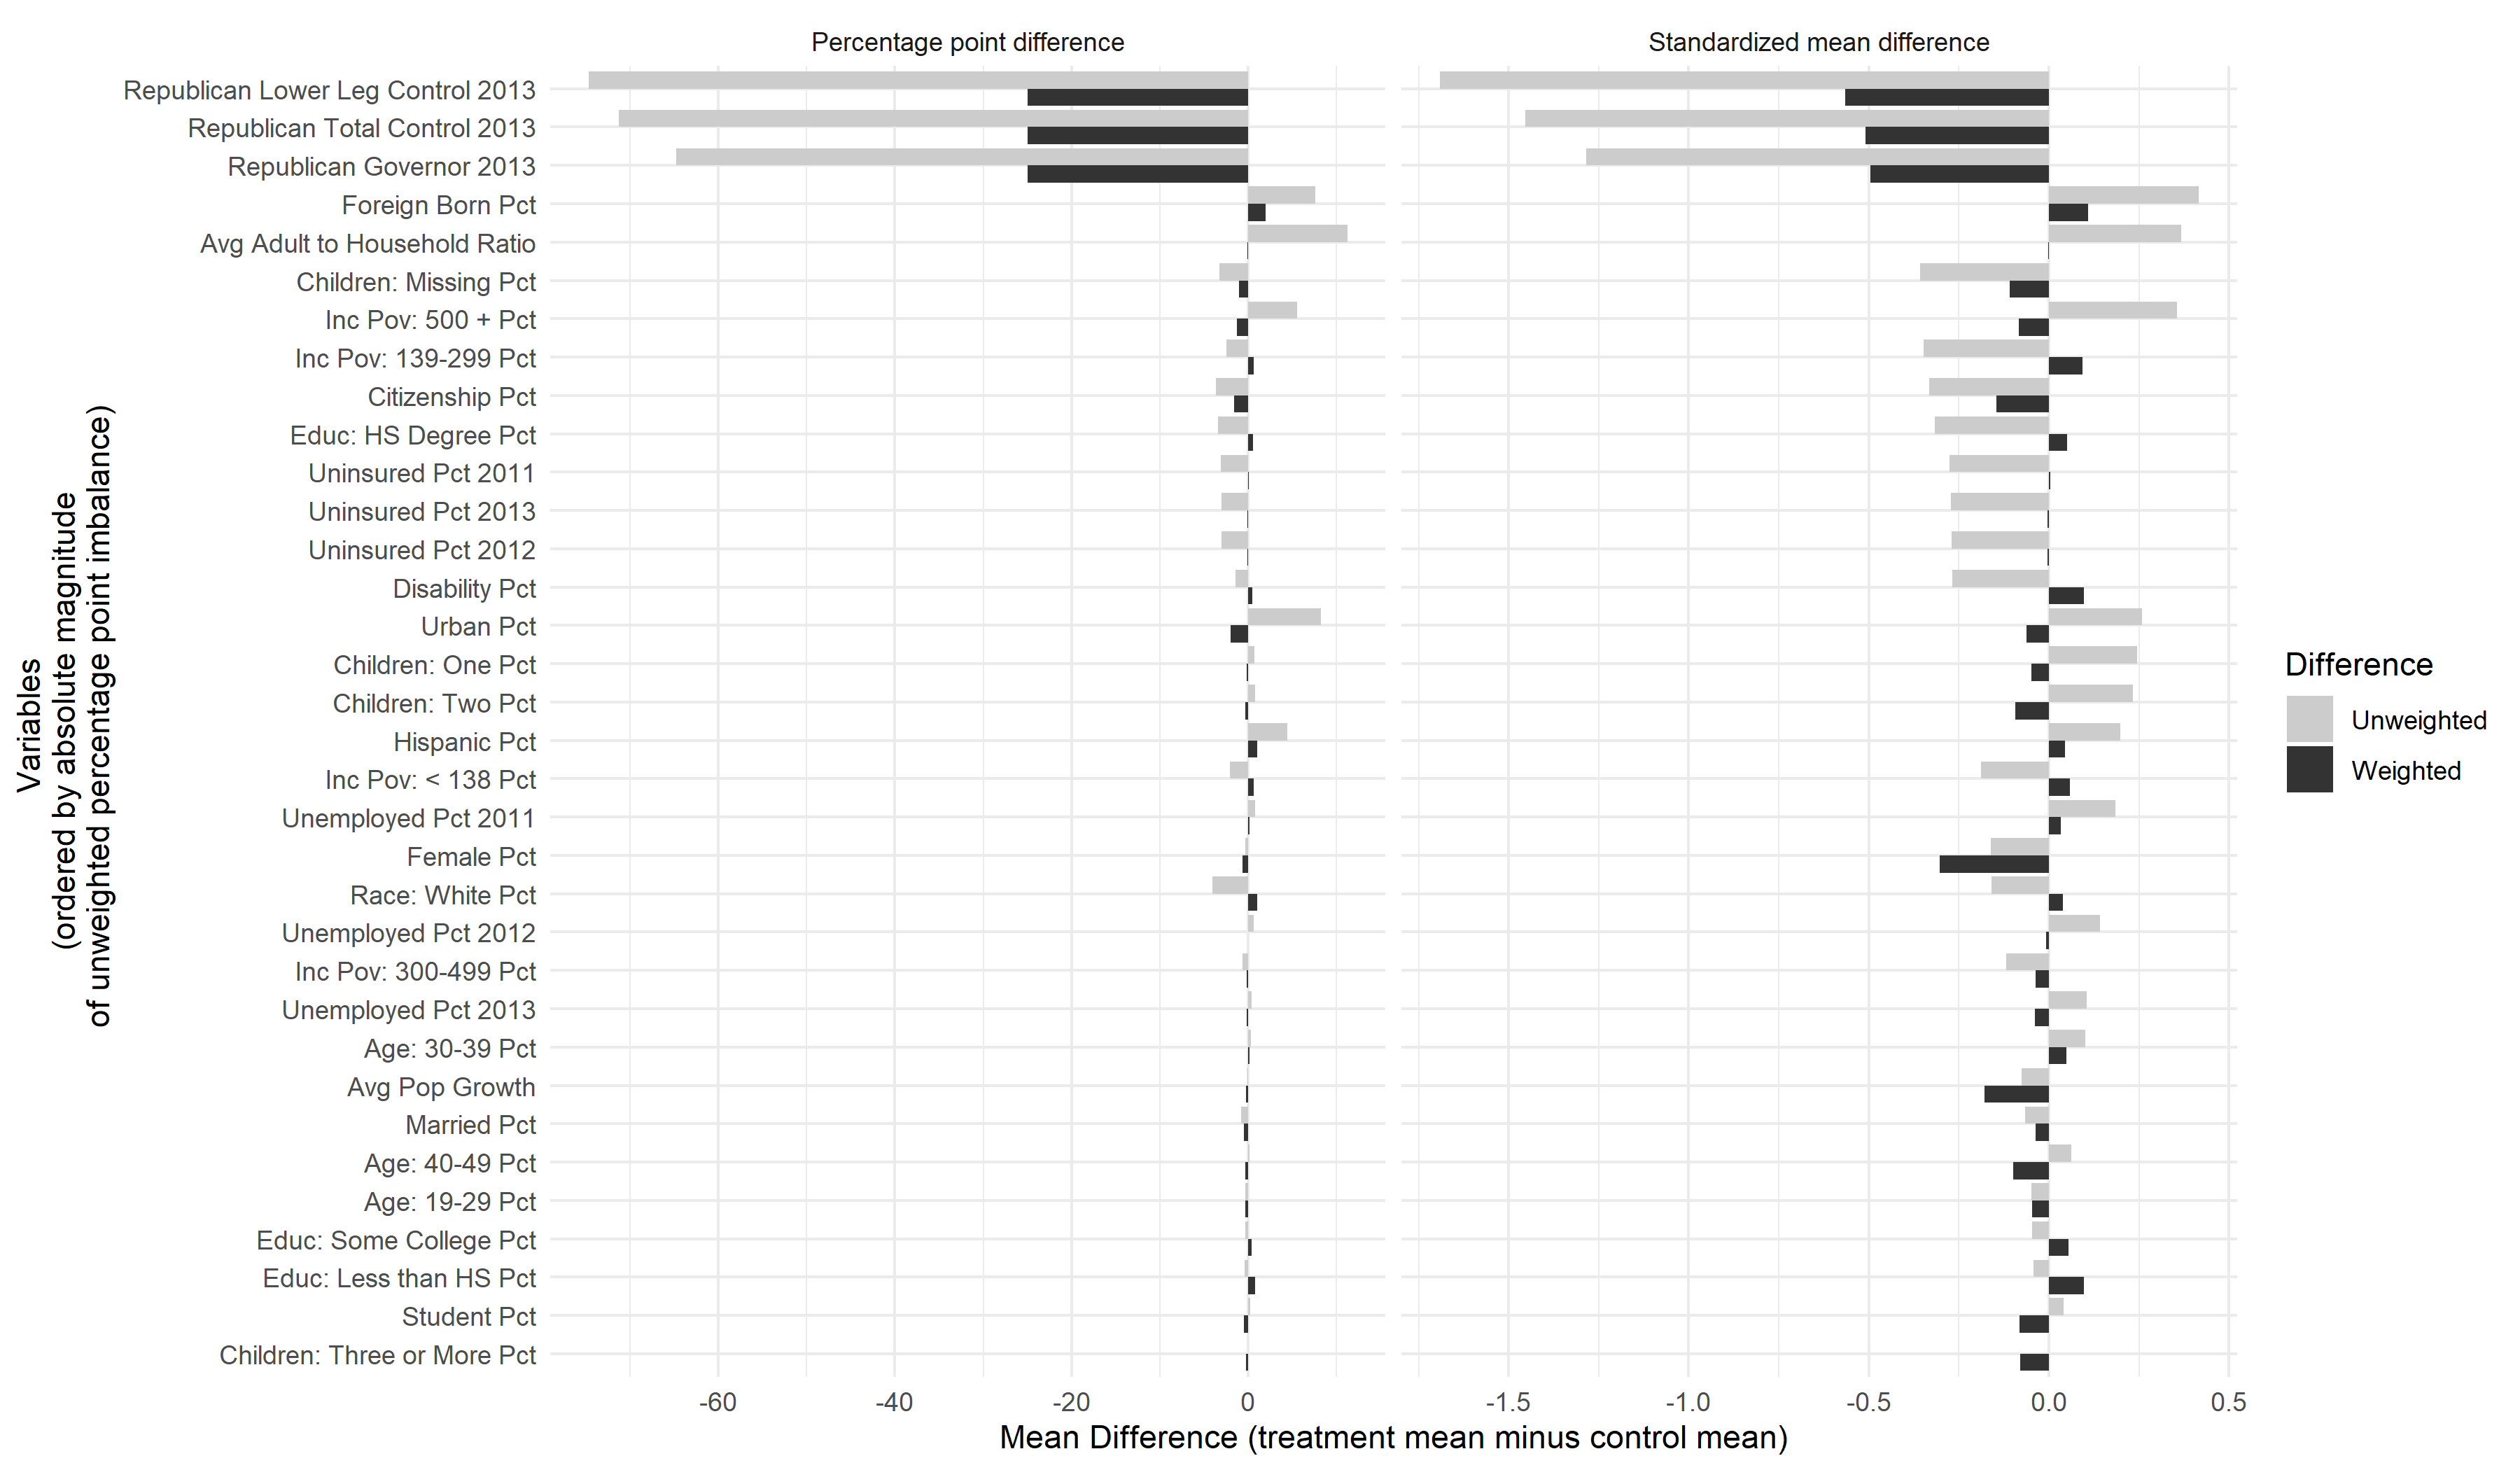
\includegraphics[scale=0.45]{01_Plots/balance-plot-all-etuc1.png}
\end{center}
\end{figure}

\begin{figure}[H]
\begin{center}
    \caption{H-SBW versus BC-HSBW versus SBW, weights summed by state, primary dataset}
    \label{fig:sbwvhsbw1}
    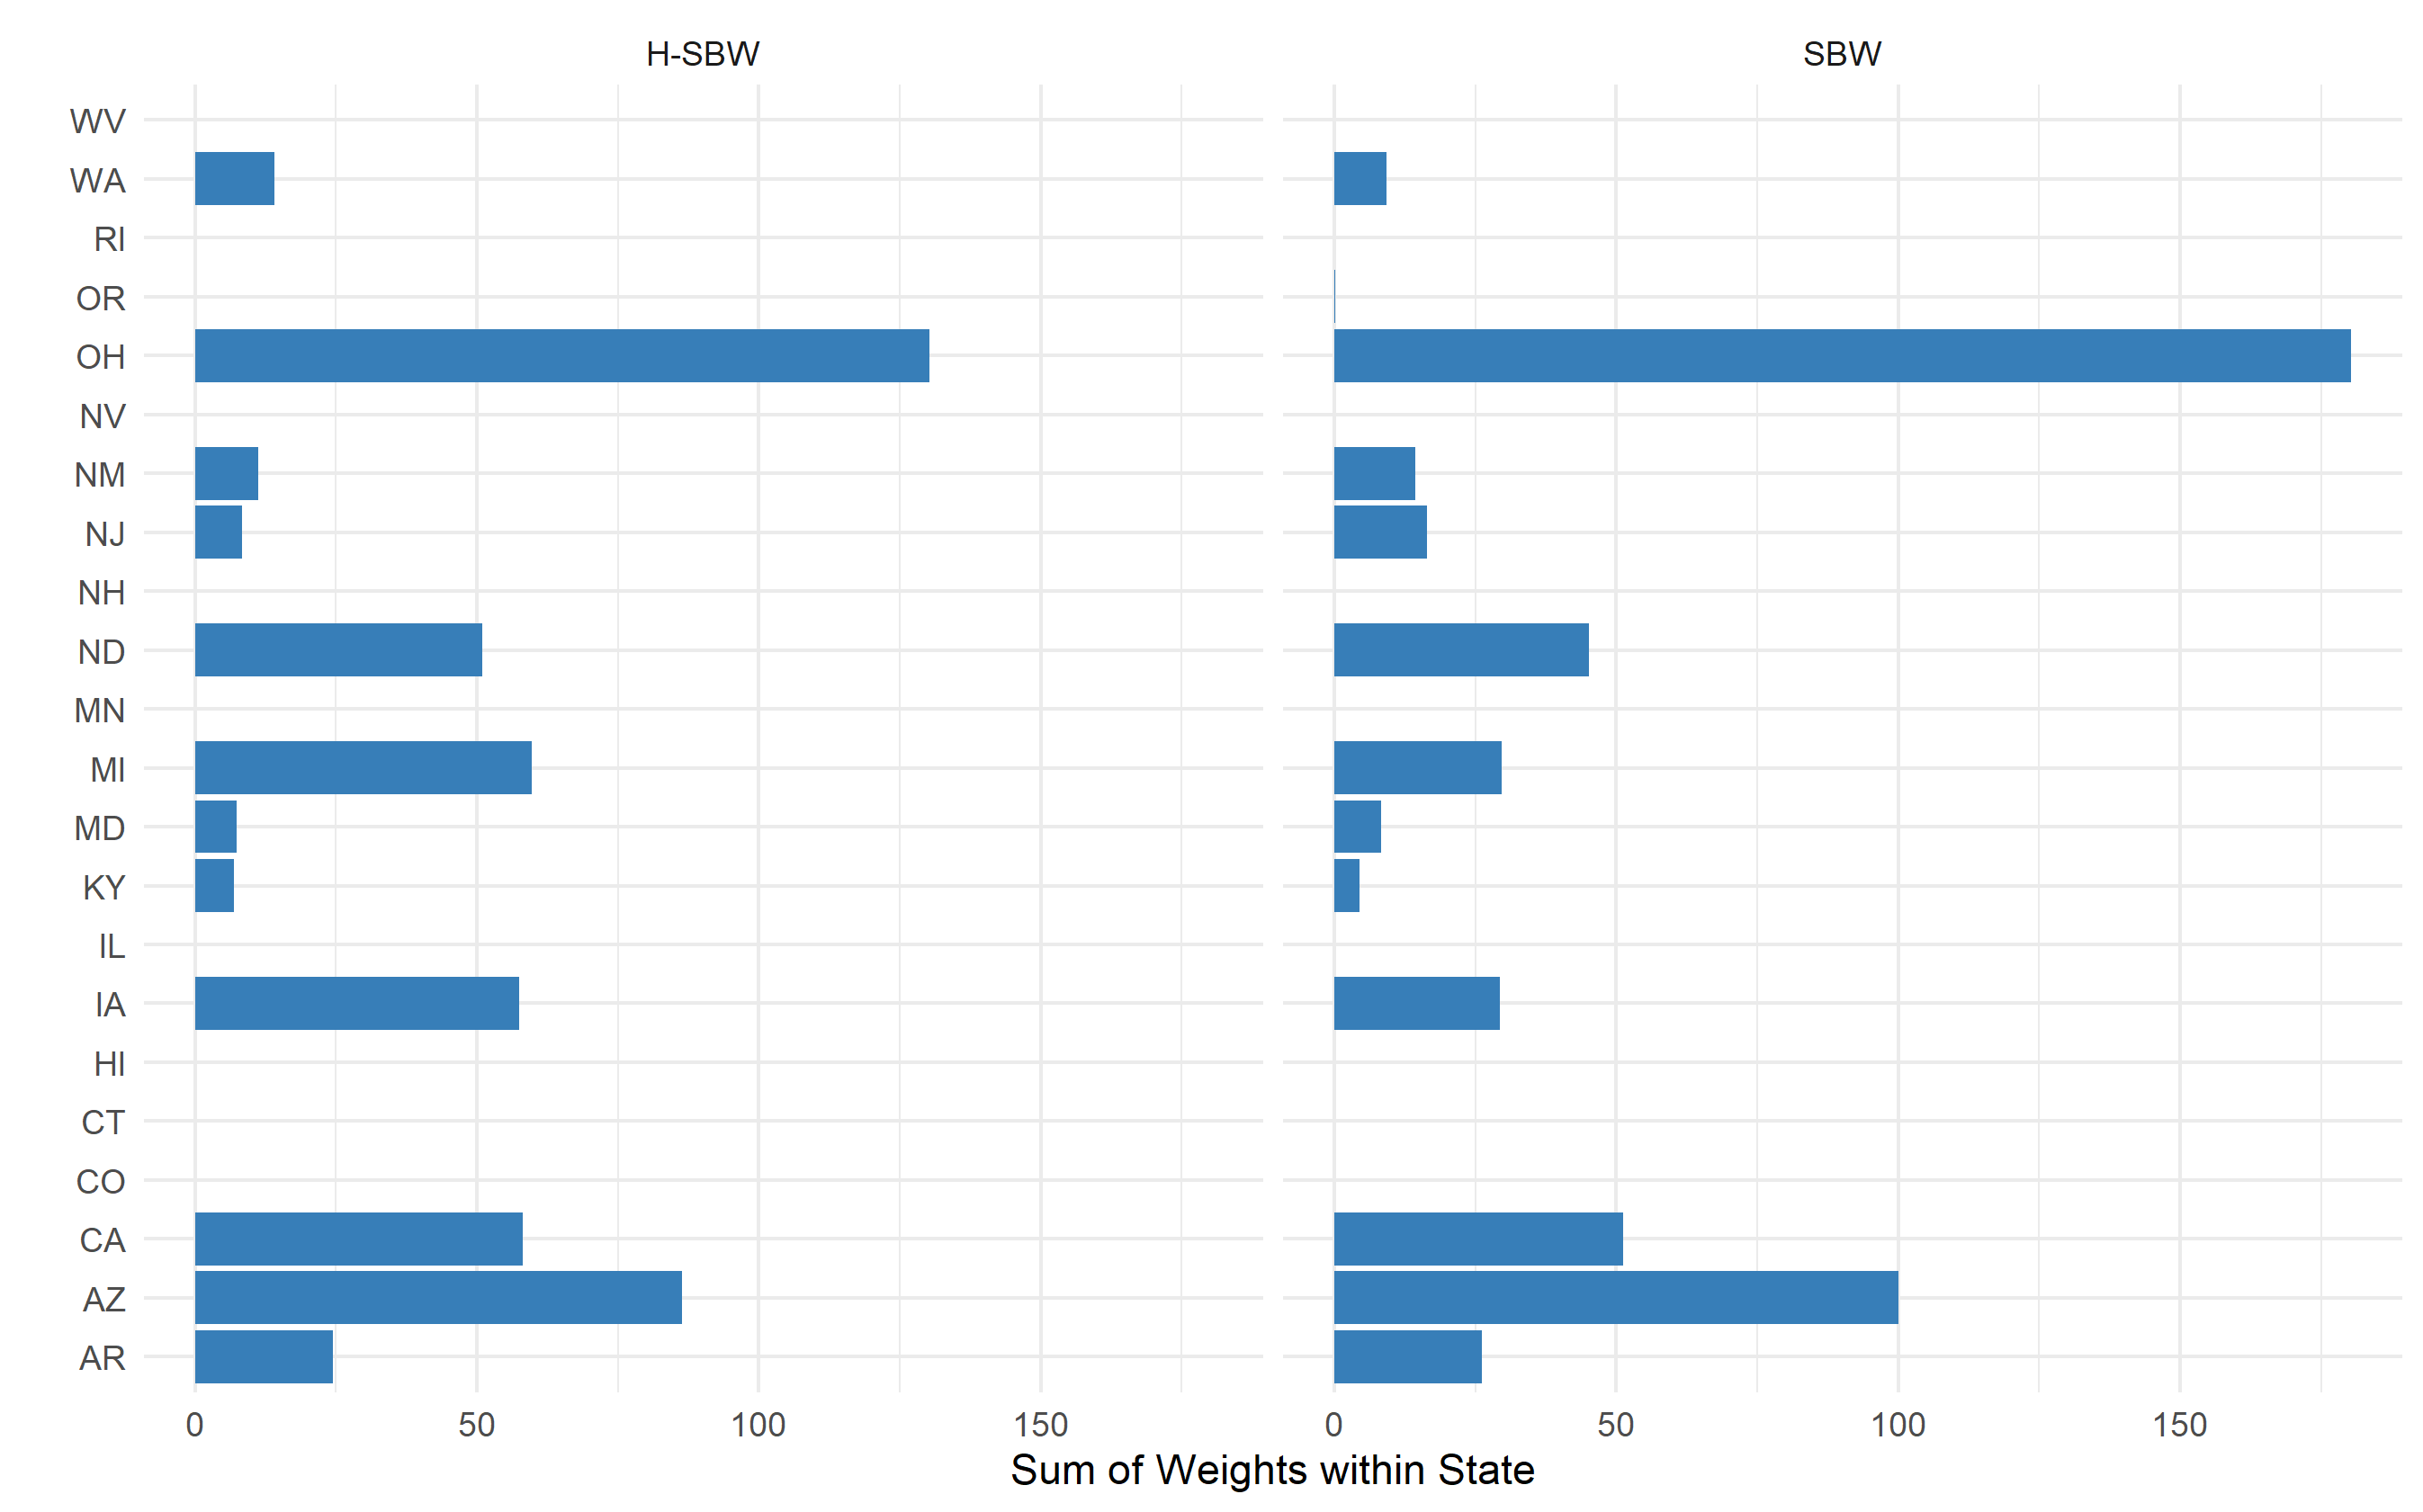
\includegraphics[scale=0.55]{01_Plots/weights-by-state-sbw-hsbw-c1.png}
\end{center}
\end{figure}

We then augment these weights using ridge-regression. Figure~\ref{fig:sbwvhsbw1} shows the total weights summed across states (and standardized to sum to 100) for three estimators: H-SBW, BC-HSBW, and SBW. For BC-HSBW we also display the sum the negative weights from the positive weights to highlight the extrapolation. This figure illustrates two key points: first, that H-SBW more evenly disperses the weights across states relative to SBW; second, that BC-HSBW extrapolates somewhat heavily in order to achieve balance, particularly from CPUMAs in California. This is likely in part because California has the most CPUMAs of any state in the dataset.

\subsection{Model validation}\label{sec:validation}

We compare the performance of our models by repeating the covariate adjustments and calculating our procedure on 2009-2011 ACS data to predict 2012 outcomes, and similarly for 2010-2012 data to predict 2013 outcomes for the non-expansion states. We run this procedure using the primary dataset and excluding the early expansion states. Table~\ref{tab:pretxpred} displays these results, with the rows ordered by RMSE of the prediction errors from the primary dataset. We see that the estimators trained on the covariate adjusted data perform substantially better than the unadjusted data and the estimators trained on the homogeneous adjustment generally outperform their counterparts on the heterogeneous adjustment. We therefore prioritize the results using the homogeneous adjustment. We also observe that H-SBW has comparable performance to SBW throughout.

Interestingly the bias-corrected estimators tend to perform relatively poorly on the primary dataset, but are the best performing estimators when excluding early expansion states -- with RMSEs lower than any other estimator on the primary dataset. As the early expansion states include California, and Figure~\ref{fig:sbwvhsbw1} shows that the bias-corrected estimators extrapolate heavily from this state, the differences in these results suggest that preventing this extrapolation may improve the model's performance. While these results do not imply that the bias-corrected models will perform poorly when predicting $\psi^1_0$ in the post-treatment period on the primary dataset (or that they will perform especially well when excluding the early expansion states), it does highlight the dangers of extrapolation: linearity may approximately hold on the support of the data where we have sufficient covariate overlap, but beyond this region this may be a more costly assumption.\footnote{In Table~\ref{tab:pretxpredfull} in Appendix~\ref{app:allresults}, we also compare the performance against the implied regression weights from OLS and GLS. These weights exactly balance the observed covariates, but are almost always the worst performing estimators in the validation study on either dataset. This also illustrates the benefits of the regularization inherent in the bias-corrected weights.}

\begin{table}[]
    \centering
\begin{longtable}{llrrrrrr}\caption{Estimator
pre-treatment outcome prediction error (in \% pts)}\label{tab:pretxpred}
 \hline
 &  & \multicolumn{3}{c}{Primary data} & \multicolumn{3}{c}{Early expansion 
 excluded} \\
 \hline
 %\cmidrule(lr){3-5} \cmidrule(lr){6-8}
Adjustment & Estimator & 2012 error & 2013 error & RMSE & 2012 error & 2013 error & RMSE \\ 
\hline
Homogeneous & SBW & -0.18 & -0.22 & 0.20 & 0.32 & -0.18 & 0.26 \\ 
Homogeneous & H-SBW & -0.24 & -0.21 & 0.23 & 0.26 & -0.24 & 0.25 \\ 
Heterogeneous & SBW & -0.25 & -0.30 & 0.27 & 0.31 & -0.24 & 0.28 \\ 
Heterogeneous & H-SBW & -0.32 & -0.39 & 0.36 & 0.25 & -0.32 & 0.29 \\ 
Homogeneous & BC-SBW & -0.42 & -0.35 & 0.39 & 0.09 & -0.15 & 0.12 \\ 
Heterogeneous & BC-SBW & -0.45 & -0.39 & 0.42 & 0.07 & -0.21 & 0.15 \\ 
Unadjusted & SBW & -0.50 & -0.61 & 0.56 & -0.18 & -0.56 & 0.42 \\ 
Unadjusted & H-SBW & -0.52 & -0.61 & 0.57 & -0.26 & -0.60 & 0.46 \\ 
Homogeneous & BC-HSBW & -0.53 & -0.62 & 0.58 & 0.05 & -0.09 & 0.07 \\ 
Heterogeneous & BC-HSBW & -0.53 & -0.72 & 0.63 & 0.03 & -0.19 & 0.14 \\ 
Unadjusted & BC-SBW & -0.82 & -0.93 & 0.88 & -0.55 & -0.84 & 0.71 \\ 
Unadjusted & BC-HSBW & -0.93 & -0.99 & 0.96 & -0.61 & -0.58 & 0.60 
 \hline
\end{longtable}
\end{table}

Finally, we observe that all estimators generated on the unadjusted dataset under-predict the true uninsurance rate. This may reflect a form of regression-to-the-mean caused by overfitting our weights to noisy covariate measurements. More formally, we can think of the uninsurance rates in time period $t$ in expansion and non-expansion regions as being drawn from separate distributions with means $(\upsilon_1, \upsilon_0)$, respectively, where $\upsilon_1 < \upsilon_0$. For simplicity assume that the only covariate in the outcome model at time $t$ is $Y_{sct-1}$. Under \eqref{eqn:linmod}, we obtain $Y_{sc} = Y_{sct} = \alpha_1 + \beta_1Y_{sct-1} + \epsilon_{sct} + \varepsilon_{st}$. The pre-treatment outcomes are likely positively correlated with the post-treatment outcomes, implying that $\beta_1 > 0$. Because $\upsilon_1 < \upsilon_0$, when reweighting the vector of noisy pre-treatment outcomes $J_{A=1}$ to $\upsilon_0$ the expected value of the weighted measurement error $\mathbb{E}[\sum_{A_{sc} = 1}\hat{\gamma}_{sc}\nu_{sct-1}]$ should be positive. In other words, our weights are likely to favor units with covariate measurements that are greater than their true covariate values. The expected value of the weighted pre-treament outcome will then be less than the target $\upsilon_0$. This implies that our estimates will be negatively biased, since $\mathbb{E}[\beta_1(\sum_{A_{sc} = 1}\hat{\gamma}_{sc}Y_{sct-1} - \upsilon_0)] \le 0$.\footnote{This phenomenon has also been discussed in the difference-in-differences and synthetic controls literature (see, e.g., \cite{daw2018matching}).} While our covariate adjustments are meant to eliminate this bias, in practice they appear more likely only to reduce it. Assuming these errors reflect a (slight) negative bias that will also hold for our estimates of $\psi^1_0$, we may expect that the true treatment effect is closer to zero than our estimates. 

\subsection{Primary Results}

Table~\ref{tab:mainresults} presents all of our estimates. Using H-SBW we estimate an effect of -2.33 (-3.54, -1.11) percentage points on our primary dataset. The SBW results are almost identical with -2.35 (-3.76, -0.95) percentage points. Compared to the unadjusted data we find very similar point estimates at -2.34 (-2.88, -1.79) percentage points for H-SBW and -2.39 (-2.99, -1.79) percentage points for SBW. We see that H-SBW reduces the confidence interval length relative to SBW on our primary dataset, though the lengths are nearly identical when excluding early expansion states. This suggests that H-SBW had at best only modest variance improvements relative to SBW in this setting. Using the adjusted covariate set also increases the length of the confidence intervals relative to the unadjusted data. This increase in the variance estimated is expected in part because the adjustment procedure generally reduces the variability in the data, as we saw in Table~\ref{tab:adjust1}, requiring that the variance of the weights to increase to achieve approximate balance. More generally this increase also reflects the uncertainty due to the measurement error.

Adding the bias-correction decreases the absolute magnitude of the estimates: we estimate effects of -2.05 (-3.30, -0.80) percentage points for BC-HSBW and -2.07 (-3.14, -1.00) percentage points for BC-SBW. This contrasts to our validation tests, where the bias-corrected estimators tended to predict lower uninsurance rates than the other estimators. The point estimates from the SBW and H-SBW estimators were virtually identical. The estimates calculated using the heterogeneous adjustment were all closer to zero than the unadjusted estimates (results are available in Appendix~\ref{app:allresults}).

\begin{table}[ht]
\begin{longtable}{lllrlr}\caption{Primary results}\label{tab:mainresults}
 \hline
 &  & \multicolumn{2}{c}{Primary data} & \multicolumn{2}{c}{Early expansion 
 excluded} \\
  \hline
Weights & Adjustment & Estimate  & Difference & Estimate & Difference\\ 
 &  & (95\% CI) &  & (95\% CI) & \\
  \hline
H-SBW & Homogeneous & -2.33 (-3.54, -1.11) & 0.01 & -2.09 (-3.24, -0.94) & 0.19 \\ 
  H-SBW & Unadjusted & -2.34 (-2.88, -1.79) & - & -2.28 (-2.87, -1.70) & - \\ 
  BC-HSBW & Homogeneous & -2.05 (-3.30, -0.80) & 0.17 & -1.94 (-3.27, -0.61) & 0.28 \\ 
  BC-HSBW & Unadjusted & -2.22 (-2.91, -1.52) & - & -2.22 (-3.14, -1.31) & - \\ 
  SBW & Homogeneous & -2.35 (-3.76, -0.95) & 0.04 & -2.05 (-3.19, -0.91) & 0.16 \\ 
  SBW & Unadjusted & -2.39 (-2.99, -1.79) & - & -2.21 (-2.75, -1.68) & - \\ 
  BC-SBW & Homogeneous & -2.07 (-3.14, -1.00) & 0.13 & -1.99 (-3.33, -0.66) & 0.23 \\ 
  BC-SBW & Unadjusted & -2.19 (-2.94, -1.45) & - & -2.23 (-3.12, -1.33) & - \\    
  \hline
\end{longtable}
\subcaption{``Difference'' column reflects difference between adjusted and unadjusted estimators}
\end{table}

All adjusted estimators were closer to zero than the corresponding unadjusted estimators. However, the difference between the adjusted SBW and H-SBW and the unadjusted versions is close to zero. This is in contrast to our validation study where the unadjusted SBW and H-SBW estimators ranged from about 0.3 to 0.4 percentage points lower than the adjusted estimators.\footnote{When excluding the early expansion states, the difference between the estimates on the adjusted and unadjusted data persist but are also smaller in magnitude.} We interpret this difference as due to chance: while theory and our validation study shows suggests that our unadjusted estimators are biased, bias only exists in expectation. Our primary dataset is a random draw where our unadjusted estimators perform more comparably to the adjusted estimators.

We next consider the sensitivity of our analysis with respect to the no anticipatory treatment effects assumption by excluding the early expansion states (California, Connecticut, Minnesota, New Jersey, and Washington) and re-running our analyses. The column ``Early excluded estimate (95\% CI)'' in Table~\ref{tab:mainresults} reflects these results. The overall patterns of the results are consistent with our primary estimates; however, our point estimates almost all move somewhat closer to zero. This may indicate that either the primary estimators have a slight negative bias, or that these estimates have a slight positive bias. Given our analysis of the validation study we view the first case as more likely. This would imply that our primary estimators reflect a lower bound on the true treatment effect. Regardless, the differences are small relative to our uncertainty estimates. Overall we view our primary results as relatively robust to the exclusion of these states. Additional diagnostics and results are available in Appendix~\ref{app:weightdiagnostics}.

\section{Discussion}

We divide our discussion into two sections: methodological considerations and policy considerations. 

\subsection{Methodological considerations and limitations}

We make multiple contributions to the literature on balancing weights. First, our estimation procedure accounts for mean-zero random noise in our covariates that is uncorrelated with the outcome errors. We modify the SBW constraint set to balance on a linear approximation to the true covariate values, applying the idea of regression calibration from the measurement error literature to the context of balancing weights. Our results illustrate the benefits of this procedure: using observed pre-treatment outcomes generated by an unknown data generating mechanism, Table~\ref{tab:pretxpred} demonstrates that our proposed estimators have better predictive performance when balancing on the adjusted covariates. This finding is consistent with concerns about overfitting to noisy covariate measurements and subsequent regression-to-the-mean.\footnote{See also \cite{daw2018matching}, who discuss this phenomenon in more detail in the context of difference-in-differences designs.}

This approach has several limitations: first, it requires access to auxiliary data with which to estimate the measurement error covariance matrix $\Sigma_{\nu}$. Many applications may not have access to such information. Even without such data, $\Sigma_{\nu}$ could also be considered a sensitivity parameter to evaluate the robustness of results to measurement error (see, e.g., \cite{huque2014impact}, \cite{illenberger2020impact}). Second, from a theoretic perspective, we require strong distributional assumptions on the covariates to consistently estimate $\psi_0^1$ using convex balancing weights. This contrasts to \cite{gleser1992importance}, who shows that the OLS estimates are consistent with only very weak distributional assumptions on the data (see also Propositions~\ref{cl8} and ~\ref{cl9} in Appendix~\ref{app:AsecI}). This relates to a third limitation: we require strong outcome modeling assumptions. Yet by preventing extrapolation, SBW and H-SBW estimates may be less sensitive than OLS estimates to these assumptions. Our validation results support this: the standard regression calibration adjustment using OLS and GLS weights performs the worst out of any methods we consider (see Table~\ref{tab:pretxpredfull} in Appendix~\ref{app:allresults}). In contrast, using regression-calibration with balancing weights -- even when allowing for limited extrapolation using ridge-augmentation -- performs better.\footnote{We also provide a suggestion of how to adapt our procedure to accommodate a basis expansion of gaussian covariates in Appendix~\ref{app:AsecI} Remark~\ref{remark:basis expansion}}. Developing methods to relax these assumptions further would be a valuable area for future work.

A final concern is that this procedure may be sub-optimal with respect to the mean-square error of our estimator. In particular, the bias induced by the measurement error decreases with the sample size used to calculate each CPUMA's covariate values, the minimum of which were over three hundred. Yet the variance of our counterfactual estimate decreases with the number of treated states. From a theoretic perspective, the variance is of a larger order than the bias, so perhaps the bias from measurement error should not be a first-order concern. Our final results support this: the changes in our results on the adjusted versus unadjusted data are of smaller magnitude than the associated uncertainty estimates. Other studies have proposed tests of whether the measurement error corrections are ``worth it'', though we do not do this here (see, e.g., \cite{gleser1992importance}). Even so, our simulation study in Appendix~\ref{app:simstudy} shows that confidence interval coverage can fall below nominal rates when using mismeasured covariates even in regimes when the measurement error is small relative to the variability in the outcome model. Using this measurement error correction can improve our ability to make valid statistical inferences in this setting even if the results are qualitatively similar.

Our second contribution is to introduce the H-SBW objective. This objective can improve upon the SBW objective assuming that the errors in the outcome model are homoskedastic with constant positive equicorrelation $\rho$ within known groups of units. Assuming no measurement error and that $\rho$ is known, we show that H-SBW returns the minimum variance estimator within the constraint set by more evenly dispersing weights across the groups. We also demonstrate the connection between these weights and the implied weights from GLS (see Propositions~\ref{cl4} and \ref{cl56} in Appendix~\ref{app:AsecII}). While studies have considered balancing weights in settings with hierarchical data (see, e.g., \cite{keele2020hospital}), we are the first to our knowledge to propose changing the criterion to account for correlated outcomes.

This estimation procedure has at least three potential drawbacks. First, we make a very specific assumption on the covariance structure of the error terms that is useful for our application. Applications where a different structure $\Omega$ is more appropriate one can still follow our approach and minimize the more general criterion $f(\gamma) = \gamma^T\Omega\gamma$. Second, we require specifying the parameters $(\rho, \delta)$ in advance. Choosing $\delta$ is a challenging problem shared with SBW and we do not offer any new suggestions.\footnote{We refer to \cite{wang2020minimal} who offer an interesting data-driven approach to this problem.} Choosing $\rho$ is a new problem of this estimation procedure. Encouragingly, our simulation study shows the H-SBW estimator for any chosen $\rho$ almost always has lower variance than SBW in the presence of state-level random effects (see Appendix~\ref{app:simstudy}).\footnote{We caution that this finding solely reflects the simulation space we examined.} Even so, identifying a principled approach to choosing this parameter would be a useful future contribution. Third, in the presence of both measurement error and dependent data, using H-SBW in combination with the standard regression-calibration adjustment may be biased. This bias arises because the standard adjustment assumes independent observations. Our simulations show that this bias can increase with $\rho$ and that SBW remains approximately unbiased if the covariates are gaussian - though H-SBW may still have modest MSE improvements. We also show a theoretical modification to the adjustment procedure so that H-SBW will return unbiased estimates in this setting (see Propositions~\ref{cl7} and ~\ref{cl7hsbw}).

\subsection{Policy considerations and limitations}

We estimate that had states that did not expand Medicaid in 2014 instead expanded their programs, they would have seen a -2.33 (-3.54, -1.11) percentage point change in the average adult uninsurance rate. Our validation study and robustness checks indicate that this estimate may be biased downwards (away from zero), in which case we can interpret this estimate as a lower bound on the ETC. Existing estimates place the ETT between -3 and -6 percentage points. These estimates vary depending on the targeted sub-population of interest, the data used, the level of modeling (individuals or regions), and the modeling approach (see, e.g., \cite{courtemanche2017early}, \cite{kaestner2017effects}, \cite{frean2017premium}). Our estimate of the ETC are closer to zero than these estimates. When we attempt to estimate the ETT using our proposed method, the resulting estimates have high uncertainty due to limited covariate overlap.\footnote{In particular, there were no states entirely controlled by Democrats that did not expand Medicaid. Even allowing for large imbalances, our standard error estimates were approximately three percentage points and our confidence intervals all contained zero. When estimating a simple difference-in-differences model on the unadjusted dataset we estimate that the ETT is -2.05 (-3.23, -0.87), where the standard errors account for clustering at the state level.\label{footnote_did}} The differences may reflect different modeling strategies and data, or it may suggest that the ETC is smaller in absolute magnitude than the ETT.

We ultimately make no formal statistical claims about these differences, but we do emphasize the importance of caution when using estimates of the ETT to make inferences about the ETC. Because almost every outcome of interest is mediated through increasing the number of insured individuals, if the ETC is in fact different than the ETT, then projecting findings from an estimate of the ETT to the ETC may lead to inaccurate inferences. For example, \cite{miller2019medicaid} study the effect of Medicaid expansion on mortality. Using their estimate of the ETT they project that had all states expanded Medicaid, 15,600 deaths would have been avoided during their study's time-period. If we believe that this number increases monotonically with the number of uninsured individuals, this estimate may be an overestimate if the ETC is less than the ETT, or an underestimate if the ETC is greater than the ETT. Directly estimating the ETC can help us better model policy relevant downstream effects mediated through changing the uninsurance rate. 

Our estimate is not without limitations. Specifically, our analysis requires many strong modeling assumptions. In particular, we require SUTVA, no anticipatory treatment effects, no unmeasured confounding conditional on the true covariates, and several parametric assumptions regarding the outcome and measurement error models. We have addressed some concerns about possible violations of these assumptions. For example, our results were qualitatively similar whether we excluded possible ``early expansion states,'' or used different weighting strategies (including relaxing the positivity restrictions and changing the tuning parameter $\rho$). However, we do not attempt to address concerns about the impact of spillovers across regions. And while we believe that no unmeasured confounding is reasonable for this problem, we did not conduct a sensitivity analysis (see, e.g., \cite{bonvini2021sensitivity}) with respect to this assumption. 

Medicaid expansion remains an ongoing policy debate in the United States, with states such as Wyoming, Alabama, and North Carolina reportedly considering expanding their programs. Our study estimates the effect of Medicaid expansion on adult uninsurance rates; however, the primary reason this effect interesting is that Medicaid enrollment is not automatic for eligible individuals. If the goal of Medicaid expansion is to increase insurance access for low-income adults, state policy-makers also may wish to make it easier or even automatic to enroll in Medicaid. 

\section{Conclusion}

We predict the average change in the non-elderly adult uninsurance rate in 2014 among states that did not expand their Medicaid eligibility thresholds as if they had. We use survey data aggregated to the CPUMA-level to estimate this quantity. The resulting dataset has both measurement error in the covariates that may bias standard estimation approaches, and a hierarchical structure that may worsen the efficiency of these same approaches. We therefore propose an estimation procedure that uses balancing weights that accounts for these problems. We demonstrate that our bias-reduction approach improves on existing methods when predicting observed outcomes from an unknown data generating mechanism. Applying this method to our problem, we estimate that states that did not expand Medicaid in 2014 would have seen a -2.33 (-3.54, -1.11) percentage point change in their adult uninsurance rates had they done so. This is the first study we are aware of that directly estimates the treatment effect on the controls with respect to Medicaid expansion. From a methodological perspective, we demonstrate the value of our proposed method relative to existing methods. From a policy-analysis perspective, we emphasize the importance of directly estimating the relevant causal quantity of interest. More generally if the goal of Medicaid expansion is to improve access to insurance, state and federal policy-makers should consider policies that make Medicaid enrollment easier if not automatic.

\section*{Acknowledgements}

The authors gratefully acknowledge invaluable advice and comments from Zachary Branson, Riccardo Fogliato, Edward Kennedy, Brian Kovak, Akshaya Jha, Lowell Taylor, and Jose Zubizaretta.

\begin{supplement}
Analysis programs and supporting materials are available online at \url{github.com /mrubinst757/medicaid-expansion}. Proofs and additional results are available in the Appendix.
\end{supplement}

\bibliographystyle{imsart-nameyear} % Style BST file
\bibliography{research.bib}       % Bibliography file (usually '*.bib')

\end{document}
